%%%%%%%%%%%%%%%%%%%%%%%%%%%%%%%%%%%%%%%%%%%%%%%%%%%%%%%%%%%%%%%%%%%%%%
%% Methods section
%% Paper: Mapping the land-use footprint of Brazilian soy embodied in
%%        international consumption -- a spatially explicit input-output
%%        approach
%% Target: Nature Portfolio (Nature Food) -- see docs/paper_plan.md
%%
%% Formulas correspond to the pipeline code (code/pipeline/00..21); only
%% load-bearing equations are displayed, routine allocations and unit
%% conversions are described in prose. The multimodal GAMS/LP variant is
%% intentionally NOT described here (currently non-runnable; mention
%% belongs in Discussion/limitations of the main manuscript).
%%
%% Uses the official Springer Nature template (sn-jnl.cls) with the
%% Nature Portfolio reference style (sn-nature). Compile with:
%%   pdflatex methods && bibtex methods && pdflatex methods && pdflatex methods
%%%%%%%%%%%%%%%%%%%%%%%%%%%%%%%%%%%%%%%%%%%%%%%%%%%%%%%%%%%%%%%%%%%%%%

\documentclass[pdflatex,sn-nature]{sn-jnl}% Nature Portfolio reference style

%%%% Standard packages
\usepackage{graphicx}%
\usepackage{amsmath,amssymb,amsfonts}%
\usepackage{amsthm}%
\usepackage{xcolor}%
\usepackage{textcomp}%
\usepackage{manyfoot}%
\usepackage{booktabs}%
\usepackage{geometry}%
\usepackage{tikz}%
\usetikzlibrary{arrows.meta,positioning,decorations.pathreplacing}

%%%% Math helpers
\DeclareMathOperator*{\argmin}{arg\,min}
\DeclareMathOperator{\diag}{diag}
\newcommand{\CBS}[2]{\mathrm{CBS}[#1,#2]}

\raggedbottom

\begin{document}

\title[Land-use footprint of Brazilian soy]{Mapping the land-use footprint
of Brazilian soy embodied in international consumption: a spatially explicit
input--output approach}

\author*[1]{\fnm{Liza} \sur{Buriak}}\email{TODO@wu.ac.at}

\affil*[1]{\orgdiv{Institute for Ecological Economics},
\orgname{Vienna University of Economics and Business (WU)},
\orgaddress{\city{Vienna}, \country{Austria}}}

\abstract{\emph{TODO --- Methods-only working document. The full abstract lives
in the main manuscript. Placeholder so the file compiles standalone.}}

\keywords{soy, land footprint, telecoupling, MRIO, FABIO, Brazil, deforestation}

\maketitle

%%%%%%%%%%%%%%%%%%%%%%%%%%%%%%%%%%%%%%%%%%%%%%%%%%%%%%%%%%%%%%%%%%%%%%
\section{Methods}\label{sec:methods}
%%%%%%%%%%%%%%%%%%%%%%%%%%%%%%%%%%%%%%%%%%%%%%%%%%%%%%%%%%%%%%%%%%%%%%

% ==================================================================
\subsection{Overview and notation}\label{subsec:overview}
% ==================================================================
We couple a subnational (municipality-level) reconstruction of Brazil's soy
supply chain with the global \textsc{fabio} physical multi-regional
input--output (MRIO) framework \cite{bruckner2019fabio}, and attribute the
resulting land-use footprint back to municipalities of origin and forward to
countries of final consumption, annually for 2010--2020. The construction
proceeds in six stages: (i)~municipal soy accounting, assembling production,
trade and domestic-use quantities for every Brazilian municipality
(Section~\ref{subsec:accounting}); (ii)~livestock-system disaggregation and
feed demand (Section~\ref{subsec:feed}); (iii)~reconciliation of the municipal
totals with national commodity balances (Section~\ref{subsec:balancing});
(iv)~allocation of physical flows between municipalities by cost-minimizing
optimal transport (Section~\ref{subsec:transport}); (v)~linkage of origin
municipalities to importing countries, with re-export disentangling
(Section~\ref{subsec:origin2consumer}); and (vi)~nesting into \textsc{fabio}
and land-use footprint accounting
(Sections~\ref{subsec:fabio}--\ref{subsec:footprint}). The resulting flows are
validated against the independent Trase supply-chain benchmark and a
pure-downscaling baseline (Section~\ref{subsec:validation}). The subnational
tracing framework generalizes the single-year (2013) open model of
Trsek~\cite{trsek2022} to an annual series; a script-level mapping of each
subsection to the released pipeline code is provided with the repository.
Figure~\ref{fig:workflow} summarizes the full pipeline.

\begin{figure}[htbp]
\centering
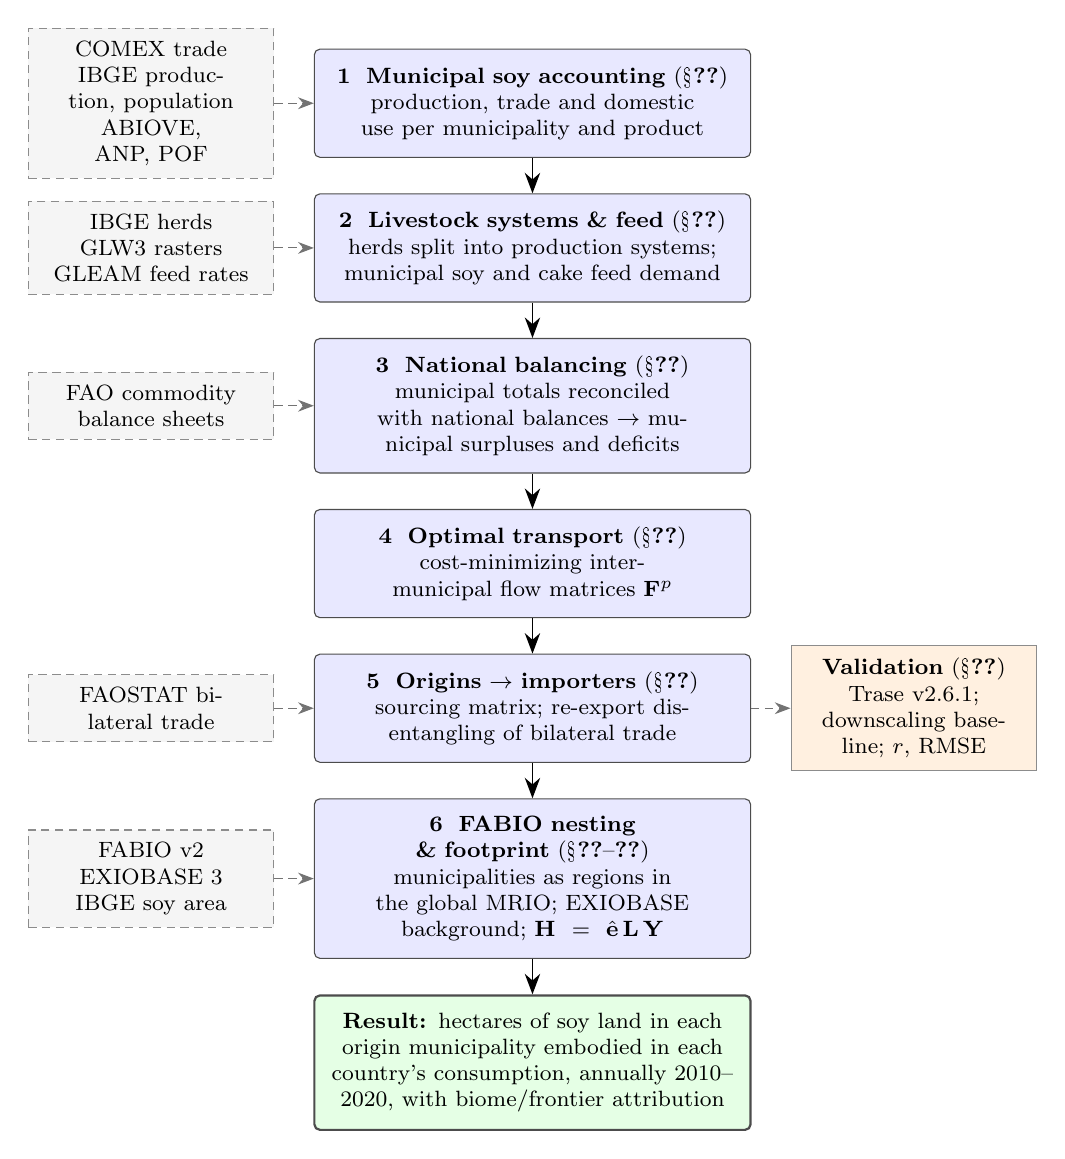
\begin{tikzpicture}[
  font=\footnotesize,
  stage/.style={draw=black!70, rounded corners=2pt, fill=blue!9,
                text width=51mm, align=center, inner sep=2.2mm},
  data/.style={draw=black!45, densely dashed, fill=black!4,
               text width=28mm, align=center, inner sep=1.6mm},
  res/.style={draw=black!70, thick, rounded corners=2pt, fill=green!10,
              text width=51mm, align=center, inner sep=2.2mm},
  val/.style={draw=black!45, fill=orange!12,
              text width=28mm, align=center, inner sep=1.6mm},
  arr/.style={-{Stealth[length=2.6mm]}, semithick},
  darr/.style={-{Stealth[length=2mm]}, densely dashed, black!55}
]
% --- main pipeline ---
\node[stage] (s1) {\textbf{1~~Municipal soy accounting}~(\S\ref{subsec:accounting})\\
  production, trade and domestic use per municipality and product};
\node[stage, below=4.5mm of s1] (s2) {\textbf{2~~Livestock systems \& feed}~(\S\ref{subsec:feed})\\
  herds split into production systems; municipal soy and cake feed demand};
\node[stage, below=4.5mm of s2] (s3) {\textbf{3~~National balancing}~(\S\ref{subsec:balancing})\\
  municipal totals reconciled with national balances $\rightarrow$
  municipal surpluses and deficits};
\node[stage, below=4.5mm of s3] (s4) {\textbf{4~~Optimal transport}~(\S\ref{subsec:transport})\\
  cost-minimizing inter-municipal flow matrices $\mathbf{F}^{p}$};
\node[stage, below=4.5mm of s4] (s5) {\textbf{5~~Origins $\rightarrow$ importers}~(\S\ref{subsec:origin2consumer})\\
  sourcing matrix; re-export disentangling of bilateral trade};
\node[stage, below=4.5mm of s5] (s6) {\textbf{6~~FABIO nesting \& footprint}~(\S\ref{subsec:fabio}--\ref{subsec:footprint})\\
  municipalities as regions in the global MRIO; EXIOBASE background;
  $\mathbf{H}=\hat{\mathbf{e}}\,\mathbf{L}\,\mathbf{Y}$};
\node[res, below=4.5mm of s6] (out) {\textbf{Result:} hectares of soy land in each origin
  municipality embodied in each country's consumption, annually 2010--2020,
  with biome/frontier attribution};
% --- data inputs (left) ---
\node[data, left=5mm of s1] (d1) {COMEX trade\\ IBGE production, population\\ ABIOVE, ANP, POF};
\node[data, left=5mm of s2] (d2) {IBGE herds\\ GLW3 rasters\\ GLEAM feed rates};
\node[data, left=5mm of s3] (d3) {FAO commodity balance sheets};
\node[data, left=5mm of s5] (d5) {FAOSTAT bilateral trade};
\node[data, left=5mm of s6] (d6) {FABIO v2\\ EXIOBASE 3\\ IBGE soy area};
% --- validation (right) ---
\node[val, right=5mm of s5] (v) {\textbf{Validation}~(\S\ref{subsec:validation})\\
  Trase v2.6.1; downscaling baseline; $r$, RMSE};
% --- arrows ---
\draw[arr] (s1) -- (s2);
\draw[arr] (s2) -- (s3);
\draw[arr] (s3) -- (s4);
\draw[arr] (s4) -- (s5);
\draw[arr] (s5) -- (s6);
\draw[arr] (s6) -- (out);
\draw[darr] (d1) -- (s1);
\draw[darr] (d2) -- (s2);
\draw[darr] (d3) -- (s3);
\draw[darr] (d5) -- (s5);
\draw[darr] (d6) -- (s6);
\draw[darr] (s5) -- (v);
\end{tikzpicture}
\caption{Workflow of the study. Solid boxes are the six model stages
(Sections~\ref{subsec:accounting}--\ref{subsec:footprint}); dashed boxes are
the main data inputs at each stage; the orange box is the independent
validation of the reconstructed flows (Section~\ref{subsec:validation}).
Stages 1--5 reconstruct Brazil's subnational soy supply chain; stage 6 embeds
it in the global FABIO/EXIOBASE input--output framework and computes the
land-use footprint.}\label{fig:workflow}
\end{figure}

\paragraph{Notation.}
Throughout, $m$ and $n$ index Brazil's $\sim$5{,}570 municipalities,
$p\in\{\text{bean},\text{oil},\text{cake}\}$ the three soy products, and
$i,j$ countries. National annual totals from the FAO commodity balance sheet
are written $\CBS{p}{\text{use}}$ --- e.g.\ $\CBS{\text{oil}}{\text{food}}$
for the national food use of soy oil. Matrices and vectors are set in bold,
$\diag(\cdot)$ denotes a diagonal matrix and $\mathbf{I}$ the identity; a hat
($\hat{\mathbf{e}}$) diagonalizes a vector.

\paragraph{The mass-conserving allocation operator.}
A single operation recurs throughout the subnational reconstruction: a
national total $T$ is distributed across municipalities in proportion to an
observable weight $w_m$,
\begin{equation}\label{eq:split}
  q_m \;=\; \frac{w_m}{\sum_{n}w_{n}}\;T,
  \qquad\text{so that}\qquad \sum_m q_m = T .
\end{equation}
The stages below differ mainly in the choice of weight $w_m$; each allocation
is verified in code against its national total. Table~\ref{tab:weights}
collects the weights used for the domestic-use items.

% ==================================================================
\subsection{Municipal soy accounting}\label{subsec:accounting}
% ==================================================================
% Pipeline step 00 (00_data_preparation) and step 01.

\subsubsection{Municipal supply, trade and infrastructure}\label{subsubsec:assemble}
Municipality-level exports and imports of the three soy products are read from
COMEX customs records, aggregated from monthly to annual tonnages, and matched
to IBGE municipality identifiers. Exports declared without a municipality of
origin are redistributed across the declared exporters of the same product and
destination in proportion to their declared volumes, which conserves national
totals by construction; undeclared imports are negligible and not
redistributed. Installed crushing and refining capacity (ABIOVE) is divided
equally among each state's active plants and summed per municipality;
grain-storage capacity is aggregated from georeferenced warehouse records; and
biodiesel capacity (ANP) is attributed to soy by each macro-region's soy
feedstock share. All geometries are projected to a planar national reference
system (SIRGAS~2000 / Brazil Polyconic, EPSG:5880), and each municipality is
represented by its seat; straight-line distances between seats later serve as
the transport costs of Section~\ref{subsec:transport}.

\subsubsection{Domestic-use estimation}\label{subsubsec:domuse}
Every domestic-use item of the national commodity balance is distributed
across municipalities with the allocation operator \eqref{eq:split}, using the
weights in Table~\ref{tab:weights}. The national soybean crush is allocated in
proportion to crushing capacity; municipal oil and cake output then follow
from the crush with conversion yields derived each year from the national
balance itself (the ratio of national oil and cake production to beans
crushed, $\approx$20\% oil and $\approx$75\% cake, with a $\approx$5\%
processing loss, consistent with literature values). Food use of beans and oil
is allocated by household soy-oil consumption, constructed as the state-level
per-capita acquisition rate (POF) times municipal population; other (biodiesel)
use by soy-attributable biodiesel capacity; seed use by soybean production;
and stock changes by storage capacity. A net national stock \emph{addition} is
carried on the use side; a net national \emph{withdrawal} is instead treated as
a component of \emph{supply} (Eq.~\ref{eq:balance}), distributed across
municipalities by the same storage weight but added to municipal supply rather
than subtracted from use. This mirrors the commodity-balance identity, in which
a drawdown is a genuine source of current-year supply, and keeps every municipal
use non-negative---as required by the re-export inversion of
Section~\ref{subsubsec:reexport}, since a storage-based split of a drawdown on
the \emph{use} side would instead push the net use of high-storage, low-use
municipalities negative.

\begin{table}[htbp]
\small
\caption{Domestic-use items as instances of the allocation operator
\eqref{eq:split}: each item is a national commodity-balance total distributed
across municipalities by the stated weight $w_m$.}\label{tab:weights}
\begin{tabular}{@{}ll@{}}
\toprule
Use item & Allocation weight $w_m$ \\
\midrule
Processing (crush)  & installed crushing capacity \\
Food (beans, oil)   & per-capita soy-oil acquisition $\times$ population \\
Other (biodiesel)   & soy-attributable biodiesel capacity \\
Seed                & soybean production \\
Stock change        & storage capacity (addition $\to$ use; withdrawal $\to$ supply) \\
\botrule
\end{tabular}
\end{table}

% ==================================================================
\subsection{Livestock systems and feed demand}\label{subsec:feed}
% ==================================================================
% Pipeline steps 02-03.
IBGE municipal herd counts are split into production systems --- extensive and
intensive chicken; extensive, intensive and industrial pig; grassland- and
mixed-based cattle and buffalo, each divided into dairy and meat --- because
soy feed intake differs strongly across systems. System shares are obtained by
area-weighted zonal statistics of the 2010 FAO gridded-livestock rasters
(GLW3) and the GLEAM ruminant production-system map over each municipality;
where a municipality reports a herd but had no gridded animals in 2010, the
state-mean share is used. Dairy herds are identified by milked-cow counts, and
feedlot cattle --- reported only in the agricultural census --- are
extrapolated from 2006 with the national confinement growth rate while holding
the municipal pattern fixed. The full split formulas are given in
Appendix~\ref{app:livestock}; each species' subsystems are verified to
partition its reported herd exactly.

Feed demand follows by multiplying each herd by its GLEAM per-animal intake:
annual dry-matter intake times the share sourced from soybeans and from soy
cake, converted to as-fed tonnes at 88\% dry-matter content. A single national
factor then rescales the resulting bottom-up totals to the FAO national feed
figures --- an application of \eqref{eq:split} with the bottom-up
municipality$\times$system feed matrix as weight --- preserving the spatial
and cross-system distribution while matching the national constraint.
Municipal feed demand for beans and cake is the sum over systems.
Figure~\ref{fig:feed} sketches the construction.

\begin{figure}[htbp]
\centering
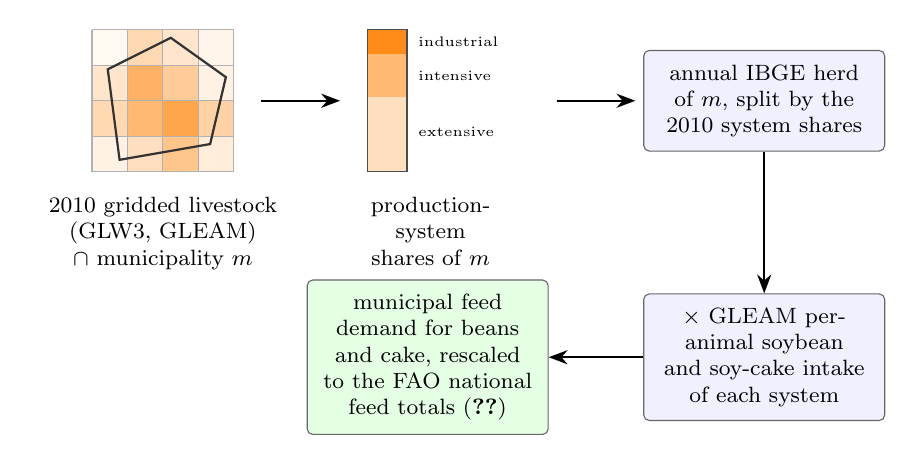
\begin{tikzpicture}[font=\footnotesize,
  box/.style={draw=black!60, rounded corners=2pt, fill=blue!6,
              text width=27mm, align=center, inner sep=1.8mm},
  arr/.style={-{Stealth[length=2.4mm]}, semithick}]
% --- raster with municipality polygon ---
\begin{scope}
\foreach \i/\j/\c in {0/0/10, 1/0/25, 2/0/45, 3/0/15,
                      0/1/30, 1/1/55, 2/1/70, 3/1/35,
                      0/2/20, 1/2/60, 2/2/40, 3/2/10,
                      0/3/5,  1/3/30, 2/3/20, 3/3/8}
  \fill[orange!\c] (\i*0.45,\j*0.45) rectangle (\i*0.45+0.45,\j*0.45+0.45);
\draw[black!30, step=0.45cm] (0,0) grid (1.8,1.8);
\draw[black!80, thick] (0.35,0.15) -- (1.5,0.35) -- (1.7,1.2)
  -- (1.0,1.7) -- (0.2,1.3) -- cycle;
\end{scope}
\node[below, text width=32mm, align=center] at (0.9,-0.2)
  {2010 gridded livestock (GLW3, GLEAM) $\cap$ municipality $m$};
\draw[arr] (2.15,0.9) -- (3.15,0.9);
% --- system-share bar ---
\begin{scope}[xshift=3.5cm]
\fill[orange!25] (0,0) rectangle (0.5,0.95);
\fill[orange!55] (0,0.95) rectangle (0.5,1.5);
\fill[orange!90] (0,1.5) rectangle (0.5,1.8);
\draw[black!70] (0,0) rectangle (0.5,1.8);
\node[right, font=\tiny] at (0.52,0.5)  {extensive};
\node[right, font=\tiny] at (0.52,1.22) {intensive};
\node[right, font=\tiny] at (0.52,1.65) {industrial};
\node[below, text width=24mm, align=center] at (0.8,-0.2)
  {production-system shares of $m$};
\end{scope}
\draw[arr] (5.9,0.9) -- (6.9,0.9);
% --- herd box ---
\node[box, anchor=west] (herd) at (7.0,0.9)
  {annual IBGE herd of $m$, split by the 2010 system shares};
% --- second row ---
\node[box, below=18mm of herd] (intake)
  {$\times$ GLEAM per-animal soybean and soy-cake intake of each system};
\node[box, fill=green!10, left=12mm of intake] (feed)
  {municipal feed demand for beans and cake, rescaled to the FAO national
   feed totals~\eqref{eq:split}};
\draw[arr] (herd) -- (intake);
\draw[arr] (intake) -- (feed);
\end{tikzpicture}
\caption{From herds to municipal soy feed demand. Municipal herd counts
(annual) are split into production systems using the shares implied by the
2010 gridded-livestock rasters within each municipality; each system's herd
is multiplied by its per-animal soy and soy-cake intake, and the bottom-up
totals are rescaled to match the national feed use reported by
FAO.}\label{fig:feed}
\end{figure}

% ==================================================================
\subsection{National balancing and trade reconciliation}\label{subsec:balancing}
% ==================================================================
% Pipeline steps 04-05.
For each product, the national commodity balance imposes the supply--use
identity
\begin{equation}\label{eq:balance}
\begin{aligned}
  \underbrace{\text{production}+\text{imports}+\text{stock withdrawal}}_{\text{supply}}
  \hspace{28mm}&\\[-1pt]
  =\;\underbrace{\text{exports}+\text{food}+\text{feed}+\text{seed}
    +\text{processing}+\text{other}}_{\text{use}}&\,.
\end{aligned}
\end{equation}
Municipal exports and imports are first harmonized with the
\textsc{fabio}/FAOSTAT bilateral trade classification (partners absent from
the bilateral trade list are collapsed into a rest-of-world aggregate); this
step aligns classifications and applies no rescaling. Any remaining
supply--use residual at the national level is absorbed into the stock term,
and each balance item is then proportionally rescaled --- again
\eqref{eq:split}, with the item's municipal distribution as weight --- so that
every municipal aggregate matches its national total exactly. Consistent with the supply--use identity~\eqref{eq:balance}, a net national
stock withdrawal is carried on the \emph{supply} side: the drawdown is
distributed across municipalities by storage capacity and added to municipal
supply, so that every municipal use remains non-negative (addition years,
carried on the use side, are unchanged). Because the model is a single annual
snapshot, tonnes supplied from a drawdown---physically grown in earlier
years---inherit the current year's soy-area intensity
(Section~\ref{subsec:footprint}); this approximation affects only the small
share of throughput met from net stock changes. Finally, each municipality's product
balance defines its surplus or deficit,
\begin{equation}\label{eq:surplus}
  \text{surplus}^p_m=\max\!\big(\text{supply}^p_m-\text{use}^p_m,\,0\big),
  \qquad
  \text{deficit}^p_m=\max\!\big(\text{use}^p_m-\text{supply}^p_m,\,0\big),
\end{equation}
which seed the inter-municipal flows of Section~\ref{subsec:transport}.

% ==================================================================
\subsection{Subnational transport allocation}\label{subsec:transport}
% ==================================================================
% Pipeline step 07 (07_transport_R.R). The multimodal GAMS/LP variant
% (steps 06/07_GAMS, transport_lp/) is intentionally not described here.
Municipal surpluses and deficits are connected by \emph{cost-minimizing
optimal transport} --- not a gravity or distance-decay model. For each product
$p$, the inter-municipal flow matrix $\mathbf{F}^p$ solves the balanced
transportation problem
\begin{equation}\label{eq:ot}
  \mathbf{F}^{p}=\argmin_{\mathbf{F}\ge0}\ \sum_{m,n}F_{mn}\,d_{mn}
  \quad\text{s.t.}\quad
  \sum_{n}F_{mn}=\text{surplus}^p_m,\ \
  \sum_{m}F_{mn}=\text{deficit}^p_n,
\end{equation}
where $d_{mn}$ is the straight-line distance between the seats of
municipalities $m$ and $n$ (the two margins are balanced beforehand by
proportionally scaling the larger one). The problem is solved exactly by the
network-simplex algorithm (R package \texttt{transport}
\cite{schuhmacher2023transport}), separately for beans, oil and cake. The
solution is a deterministic, mass-conserving flow matrix whose margins
reproduce the municipal surpluses and deficits by construction; its adequacy
is assessed against the independent Trase benchmark in
Section~\ref{subsec:validation}. Figure~\ref{fig:flows} illustrates how
municipal balances turn into inter-municipal flows.

\begin{figure}[htbp]
\centering
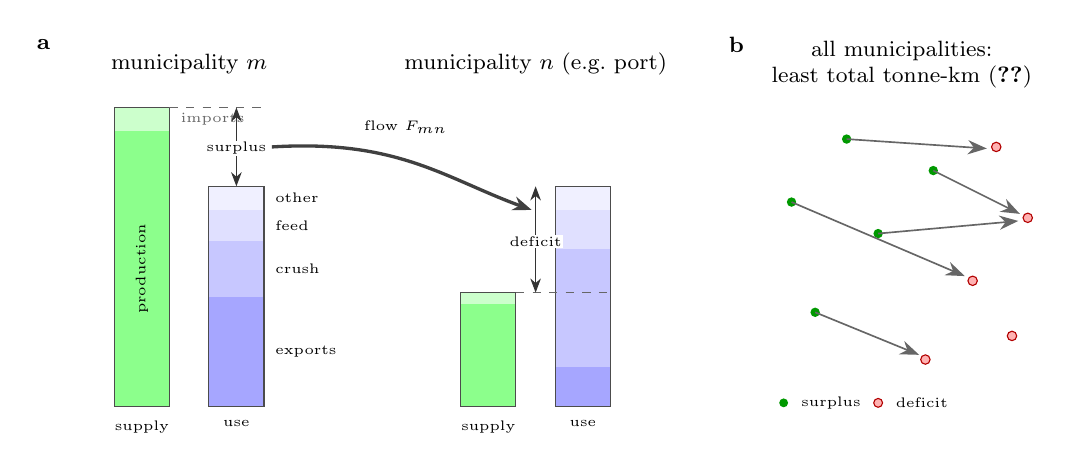
\begin{tikzpicture}[font=\footnotesize,
  arr/.style={-{Stealth[length=2.4mm]}, semithick}]
% ================= panel a: two municipal balances =================
\node[font=\footnotesize\bfseries] at (-0.9,4.6) {a};
% --- municipality m (surplus) ---
\node[align=center] at (0.95,4.35) {municipality $m$};
% supply bar
\fill[green!45] (0,0) rectangle (0.7,3.5);
\fill[green!20] (0,3.5) rectangle (0.7,3.8);
\draw[black!70]  (0,0) rectangle (0.7,3.8);
\node[font=\tiny, rotate=90] at (0.35,1.75) {production};
\node[font=\tiny, right, black!60] at (0.72,3.65) {imports};
% use bar
\fill[blue!35] (1.2,0)   rectangle (1.9,1.4);
\fill[blue!22] (1.2,1.4) rectangle (1.9,2.1);
\fill[blue!12] (1.2,2.1) rectangle (1.9,2.5);
\fill[blue!6]  (1.2,2.5) rectangle (1.9,2.8);
\draw[black!70](1.2,0)   rectangle (1.9,2.8);
\node[font=\tiny, right] at (1.92,0.7)  {exports};
\node[font=\tiny, right] at (1.92,1.75) {crush};
\node[font=\tiny, right] at (1.92,2.3)  {feed};
\node[font=\tiny, right] at (1.92,2.65) {other};
% surplus gap
\draw[dashed, black!60] (0.7,3.8) -- (1.9,3.8);
\draw[{Stealth[length=1.8mm]}-{Stealth[length=1.8mm]}, black!80]
  (1.55,2.8) -- (1.55,3.8);
\node[font=\tiny, align=center, fill=white, inner sep=0.5pt] at (1.55,3.28)
  {surplus};
\node[font=\tiny, below] at (0.35,-0.05) {supply};
\node[font=\tiny, below] at (1.55,-0.05) {use};
% --- municipality n (deficit) ---
\begin{scope}[xshift=4.4cm]
\node[align=center, font=\footnotesize] at (0.95,4.35)
  {municipality $n$ (e.g.\ port)};
\fill[green!45] (0,0) rectangle (0.7,1.3);
\fill[green!20] (0,1.3) rectangle (0.7,1.45);
\draw[black!70]  (0,0) rectangle (0.7,1.45);
\fill[blue!35] (1.2,0)   rectangle (1.9,0.5);
\fill[blue!22] (1.2,0.5) rectangle (1.9,2.0);
\fill[blue!12] (1.2,2.0) rectangle (1.9,2.5);
\fill[blue!6]  (1.2,2.5) rectangle (1.9,2.8);
\draw[black!70](1.2,0)   rectangle (1.9,2.8);
\draw[dashed, black!60] (0.7,1.45) -- (1.9,1.45);
\draw[{Stealth[length=1.8mm]}-{Stealth[length=1.8mm]}, black!80]
  (0.95,1.45) -- (0.95,2.8);
\node[font=\tiny, align=center, fill=white, inner sep=0.5pt] at (0.95,2.1)
  {deficit};
\node[font=\tiny, below] at (0.35,-0.05) {supply};
\node[font=\tiny, below] at (1.55,-0.05) {use};
\end{scope}
% flow arrow between them
\draw[arr, very thick, black!75] (2.0,3.3) .. controls (3.6,3.4) and (4.2,2.9)
  .. (5.3,2.5);
\node[font=\tiny, above] at (3.7,3.35) {flow $F_{mn}$};
% ================= panel b: optimal transport =================
\begin{scope}[xshift=8.4cm]
\node[font=\footnotesize\bfseries] at (-0.5,4.6) {b};
\node[align=center, text width=36mm] at (1.6,4.35)
  {all municipalities:\\ least total tonne-km \eqref{eq:ot}};
% surplus dots (green)
\foreach \x/\y in {0.2/2.6, 0.9/3.4, 1.3/2.2, 0.5/1.2, 2.0/3.0}
  \fill[green!60!black] (\x,\y) circle (1.7pt);
% deficit dots (red)
\foreach \x/\y in {2.8/3.3, 2.5/1.6, 3.2/2.4, 1.9/0.6, 3.0/0.9}
  \draw[red!70!black, fill=red!30] (\x,\y) circle (1.7pt);
% flows (an optimal plan on straight-line costs never crosses)
\draw[arr, black!60] (0.9,3.4) -- (2.68,3.28);
\draw[arr, black!60] (2.0,3.0) -- (3.1,2.45);
\draw[arr, black!60] (1.3,2.2) -- (3.08,2.36);
\draw[arr, black!60] (0.2,2.6) -- (2.4,1.66);
\draw[arr, black!60] (0.5,1.2) -- (1.82,0.66);
% legend
\fill[green!60!black] (0.1,0.05) circle (1.6pt);
\node[font=\tiny, right] at (0.2,0.05) {surplus};
\draw[red!70!black, fill=red!30] (1.3,0.05) circle (1.6pt);
\node[font=\tiny, right] at (1.4,0.05) {deficit};
\end{scope}
\end{tikzpicture}
\caption{From municipal balances to inter-municipal flows.
\textbf{a}, After balancing, each municipality's supply (production, imports)
and use (exports, crush, feed, food, seed) differ by a surplus or a deficit
(Eq.~\ref{eq:surplus}). Deficit municipalities are typically ports and
crushing hubs, whose exports and processing exceed local production.
\textbf{b}, Optimal transport connects all surpluses to all deficits with the
least total tonne-kilometres, yielding the flow matrix $\mathbf{F}^p$ for
each product; on straight-line costs an optimal plan contains no crossing
flows.}\label{fig:flows}
\end{figure}

% ==================================================================
\subsection{From origins to consumers}\label{subsec:origin2consumer}
% ==================================================================
% Pipeline steps 08 and 12.

\subsubsection{Linking origin municipalities to importing countries}\label{subsubsec:exportlink}
The flow matrix is converted into \emph{sourcing shares}: the fraction of
municipality $n$'s throughput that originated in municipality $m$,
\begin{equation}\label{eq:sourcing}
  \phi^p_{mn}=\frac{F^p_{mn}}{\sum_{m'}F^p_{m'n}} .
\end{equation}
Combining the sourcing shares with the observed exports $E^p_{nj}$ of
municipality $n$ to country $j$ (with a synthetic domestic column carrying
local consumption) attributes every exported tonne to its municipality of
origin,
\begin{equation}\label{eq:src2exp}
  X^p_{mj}=\delta^p_m\sum_{n}\phi^p_{mn}\,E^p_{nj},
\end{equation}
where $\delta^p_m$ --- the share of municipality $m$'s supply that is its own
production --- retains only domestically produced quantities. Oil and cake are
traced one step further back to the bean-producing municipalities by applying
the bean sourcing shares to their crush inputs.

\subsubsection{Re-export disentangling}\label{subsubsec:reexport}
To attribute internationally traded soy to its true origin, bilateral trade is
disentangled with a Leontief-type inversion. For each commodity, let
$\mathbf{T}$ be the bilateral trade matrix --- with Brazil replaced by its
municipalities for the soy products --- and $\mathbf{u}$ the vector of total
use by region. Normalizing trade by destination use and summing the infinite
re-export chain,
\begin{equation}\label{eq:reex}
  \mathbf{R}=\mathbf{T}\,\hat{\mathbf{u}}^{-1},
  \qquad
  \mathbf{L}_{\mathrm{trade}}=(\mathbf{I}-\mathbf{R})^{-1}
  =\sum_{k=0}^{\infty}\mathbf{R}^{k},
\end{equation}
and retaining only domestically produced quantities (via each region's
domestic-supply share) scaled by each destination's domestic use, yields the
origin-to-consumption matrix whose entry gives the quantity produced in region
(or municipality) $i$ and ultimately consumed in region $j$. By construction
its row and column sums recover each region's domestic supply and domestic
use.\footnote{For the soy products the region dimension comprises
non-Brazilian trade countries plus Brazilian municipalities, with national
Brazil fully replaced by its municipalities. The implementation re-asserts
this replacement after every trade-data join and verifies the dimensional
alignment of the inversion explicitly, so that no national-Brazil record can
re-enter.} Figure~\ref{fig:reexport} illustrates the correction for a
stylized example.

\begin{figure}[htbp]
\centering
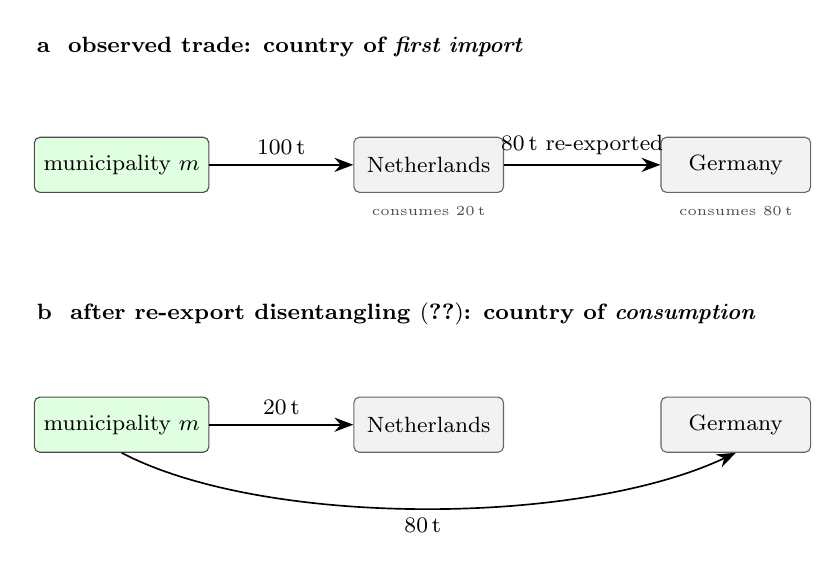
\begin{tikzpicture}[font=\footnotesize,
  cty/.style={draw=black!60, rounded corners=2pt, fill=black!5,
              minimum width=19mm, minimum height=7mm, align=center},
  mun/.style={draw=black!70, rounded corners=2pt, fill=green!12,
              minimum width=19mm, minimum height=7mm, align=center},
  arr/.style={-{Stealth[length=2.4mm]}, semithick}]
% --- observed trade ---
\node[font=\footnotesize\bfseries, anchor=west] at (-0.4,1.5)
  {a~~observed trade: country of \emph{first import}};
\node[mun] (m1) at (0.8,0) {municipality $m$};
\node[cty] (nl1) at (4.7,0) {Netherlands};
\node[cty] (de1) at (8.6,0) {Germany};
\draw[arr] (m1) -- node[above]{100\,t} (nl1);
\draw[arr] (nl1) -- node[above]{80\,t re-exported} (de1);
\node[below=0.5mm of nl1, font=\tiny, text=black!70] {consumes 20\,t};
\node[below=0.5mm of de1, font=\tiny, text=black!70] {consumes 80\,t};
% --- after inversion ---
\node[font=\footnotesize\bfseries, anchor=west] at (-0.4,-1.9)
  {b~~after re-export disentangling \eqref{eq:reex}: country of \emph{consumption}};
\node[mun] (m2) at (0.8,-3.3) {municipality $m$};
\node[cty] (nl2) at (4.7,-3.3) {Netherlands};
\node[cty] (de2) at (8.6,-3.3) {Germany};
\draw[arr] (m2) -- node[above]{20\,t} (nl2);
\draw[arr] (m2.south) .. controls (2.6,-4.6) and (6.6,-4.6) ..
  node[below]{80\,t} (de2.south);
\end{tikzpicture}
\caption{Re-export disentangling. \textbf{a}, Customs records attribute all
100\,t exported by municipality $m$ to the Netherlands, the country of first
import, although 80\,t are re-exported and consumed in Germany.
\textbf{b}, The trade inversion \eqref{eq:reex} sums re-export chains of any
length and reattributes each tonne to its country of final consumption,
leaving only the 20\,t actually consumed in the Netherlands attributed
there.}\label{fig:reexport}
\end{figure}

% ==================================================================
\subsection{Nesting into FABIO}\label{subsec:fabio}
% ==================================================================
% Pipeline steps 13-19.
The reconstructed municipal soy flows are embedded in the \textsc{fabio}~v2
physical MRIO, in which a \emph{process} is a region$\times$commodity unit.
Brazil's national soy commodities and processes are removed and replaced by
their municipal counterparts throughout, so that municipalities enter the
global model as additional regions. Figure~\ref{fig:nesting} illustrates the
nesting and the role of the Leontief inverses used below.

\begin{figure}[htbp]
\centering
% --- panel a: how municipal Brazil is inserted into the FABIO process list ---
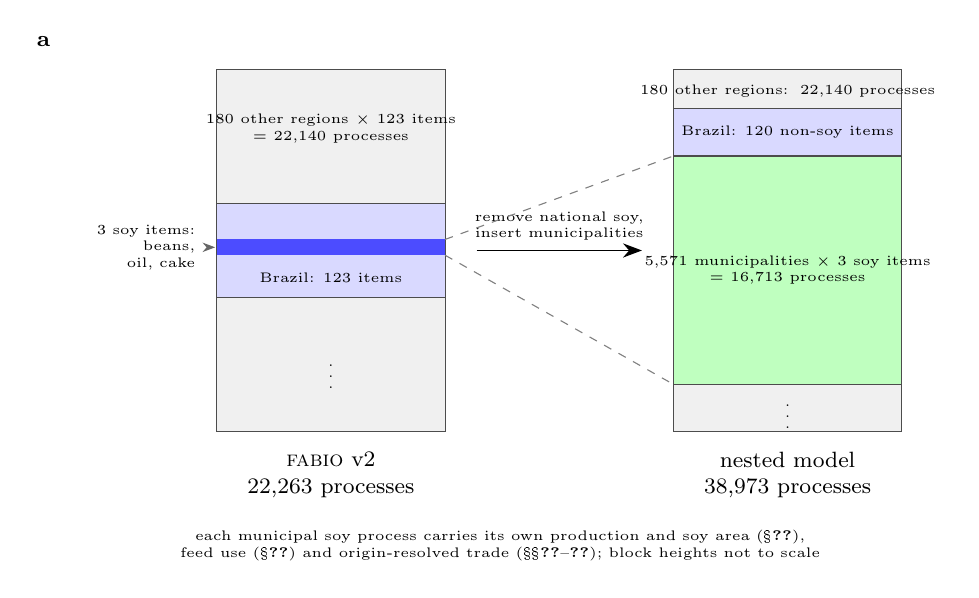
\begin{tikzpicture}[font=\footnotesize,
  arr/.style={-{Stealth[length=2.4mm]}, semithick},
  brc/.style={decorate, decoration={brace, amplitude=3pt}, black!60},
  dimlab/.style={font=\tiny, black!70, align=left}]
\node[font=\footnotesize\bfseries] at (-2.2,4.95) {a};
% ---- left column: original FABIO process list ----
\draw[fill=black!6, draw=black!70] (0,0) rectangle (2.9,4.6);
\fill[blue!15] (0,1.7) rectangle (2.9,2.9);
\fill[blue!70] (0,2.24) rectangle (2.9,2.44); % national soy stripe
\draw[black!70] (0,1.7) rectangle (2.9,2.9);
\node[font=\tiny, align=center] at (1.45,3.85)
  {180 other regions $\times$ 123 items\\ $=$ 22{,}140 processes};
\node[font=\tiny] at (1.45,1.95) {Brazil: 123 items};
\node[font=\tiny] at (1.45,0.8) {\vdots};
\node[font=\tiny, anchor=east, align=right, text width=15mm] at (-0.15,2.34)
  {3 soy items: beans, oil, cake};
\draw[-{Stealth[length=1.6mm]}, black!60] (-0.12,2.34) -- (-0.02,2.34);
\node[align=center] at (1.45,-0.55) {\textsc{fabio} v2\\ 22{,}263 processes};
% ---- arrow ----
\draw[arr] (3.3,2.3) -- node[above, align=center, text width=22mm, font=\tiny]
  {remove national soy, insert municipalities} (5.4,2.3);
% ---- right column: nested process list ----
\draw[fill=black!6, draw=black!70] (5.8,0) rectangle (8.7,4.6);
\fill[blue!15] (5.8,3.5) rectangle (8.7,4.1);
\draw[black!70] (5.8,3.5) rectangle (8.7,4.1);
\fill[green!25] (5.8,0.6) rectangle (8.7,3.5);
\draw[black!70] (5.8,0.6) rectangle (8.7,3.5);
\node[font=\tiny, align=center] at (7.25,4.32) {180 other regions:\, 22{,}140 processes};
\node[font=\tiny, align=center] at (7.25,3.8) {Brazil: 120 non-soy items};
\node[font=\tiny, align=center] at (7.25,2.05)
  {5{,}571 municipalities $\times$ 3 soy items\\ $=$ 16{,}713 processes};
\node[font=\tiny] at (7.25,0.3) {\vdots};
\node[align=center] at (7.25,-0.55) {nested model\\ 38{,}973 processes};
% zoom lines from national soy stripe to municipal block
\draw[dashed, black!50] (2.9,2.44) -- (5.8,3.5);
\draw[dashed, black!50] (2.9,2.24) -- (5.8,0.6);
% data provenance (below panel)
\node[align=center, font=\tiny, text width=112mm] at (3.6,-1.45)
  {each municipal soy process carries its own production and soy area
   (\S\ref{subsec:accounting}), feed use (\S\ref{subsec:feed}) and
   origin-resolved trade
   (\S\S\ref{subsec:transport}--\ref{subsec:origin2consumer});
   block heights not to scale};
\end{tikzpicture}

\vspace{4mm}

% --- panel b: hybrid coefficient matrix with municipal nesting ---
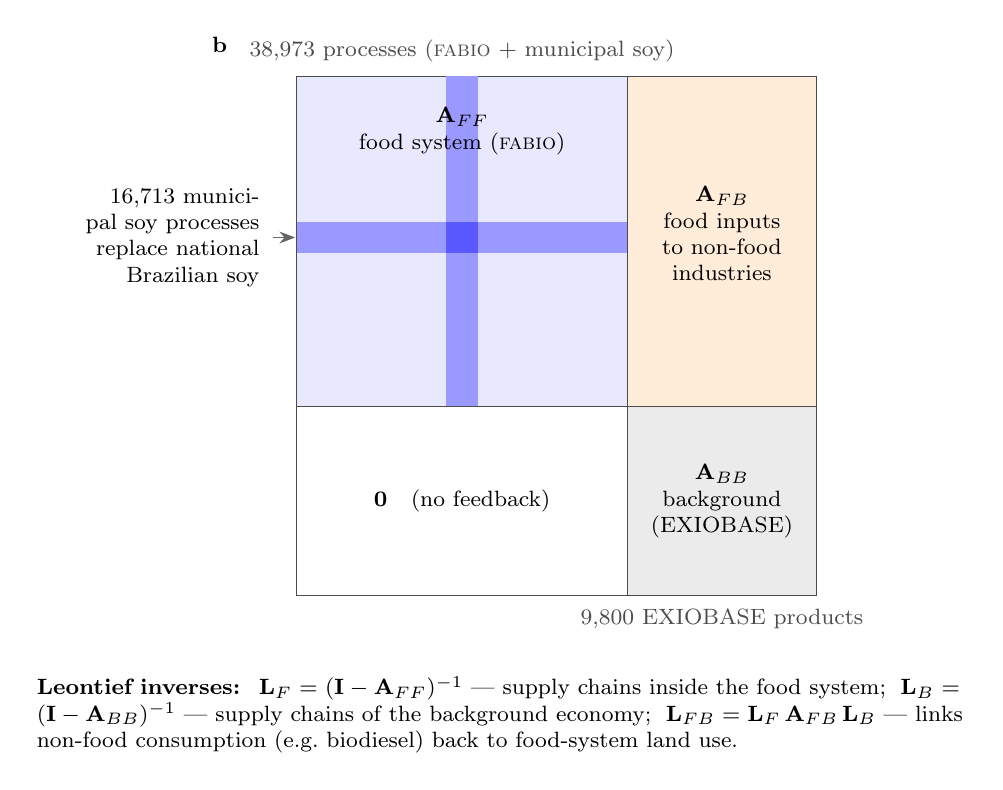
\begin{tikzpicture}[font=\footnotesize]
\node[anchor=west, font=\footnotesize\bfseries] at (-1.2,7.0) {b};
% A_FF block
\draw[fill=blue!9, draw=black!70] (0,2.4) rectangle (4.2,6.6);
% municipal rows band
\draw[fill=blue!40, draw=none] (0,4.35) rectangle (4.2,4.75);
% municipal cols band
\draw[fill=blue!40, draw=none] (1.9,2.4) rectangle (2.3,6.6);
\draw[fill=blue!65, draw=none] (1.9,4.35) rectangle (2.3,4.75);
\node[align=center] at (2.1,5.9) {$\mathbf{A}_{FF}$\\ food system (\textsc{fabio})};
% A_FB block
\draw[fill=orange!15, draw=black!70] (4.2,2.4) rectangle (6.6,6.6);
\node[align=center] at (5.4,4.6) {$\mathbf{A}_{FB}$\\ food inputs\\ to non-food\\ industries};
% zero block
\draw[fill=white, draw=black!70] (0,0) rectangle (4.2,2.4);
\node at (2.1,1.2) {$\mathbf{0}$\quad(no feedback)};
% A_BB block
\draw[fill=black!8, draw=black!70] (4.2,0) rectangle (6.6,2.4);
\node[align=center] at (5.4,1.2) {$\mathbf{A}_{BB}$\\ background\\ (EXIOBASE)};
% municipal annotation
\draw[-{Stealth[length=2mm]}, black!60] (-0.3,4.55) -- (-0.02,4.55);
\node[align=right, anchor=east, text width=24mm] at (-0.35,4.55)
  {16{,}713 municipal soy processes replace national Brazilian soy};
% dimensions
\node[black!70, above] at (2.1,6.65) {38{,}973 processes (\textsc{fabio} $+$ municipal soy)};
\node[black!70, below] at (5.4,-0.05) {9{,}800 EXIOBASE products};
% inverse summary (below matrix)
\node[align=left, anchor=north, text width=118mm] at (2.6,-0.9)
  {\textbf{Leontief inverses:}\;
   $\mathbf{L}_F=(\mathbf{I}-\mathbf{A}_{FF})^{-1}$ --- supply chains inside
   the food system;\;
   $\mathbf{L}_B=(\mathbf{I}-\mathbf{A}_{BB})^{-1}$ --- supply chains of the
   background economy;\;
   $\mathbf{L}_{FB}=\mathbf{L}_F\,\mathbf{A}_{FB}\,\mathbf{L}_B$ --- links
   non-food consumption (e.g.\ biodiesel) back to food-system land use.};
\end{tikzpicture}

\vspace{4mm}

% --- panel c: what the inverse does (one example chain) ---
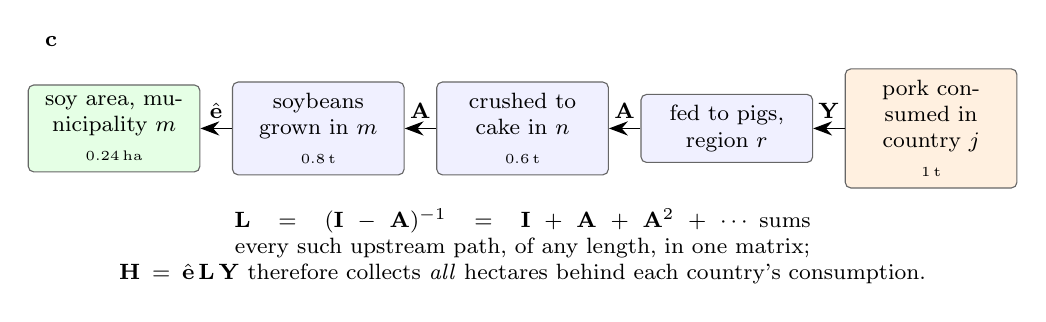
\begin{tikzpicture}[font=\footnotesize,
  box/.style={draw=black!60, rounded corners=2pt, fill=blue!6,
              text width=19mm, align=center, inner sep=1.4mm},
  arr/.style={-{Stealth[length=2.4mm]}, semithick}]
\node[anchor=west, font=\footnotesize\bfseries] at (-1.0,1.1) {c};
\node[box, fill=green!10] (land) {soy area, municipality $m$\\[1pt]{\tiny 0.24\,ha}};
\node[box, right=4mm of land] (bean) {soybeans grown in $m$\\[1pt]{\tiny 0.8\,t}};
\node[box, right=4mm of bean] (crush) {crushed to cake in $n$\\[1pt]{\tiny 0.6\,t}};
\node[box, right=4mm of crush] (pig) {fed to pigs, region $r$};
\node[box, right=4mm of pig, fill=orange!12] (dem) {pork consumed in country $j$\\[1pt]{\tiny 1\,t}};
\draw[arr] (dem) -- node[above]{$\mathbf{Y}$} (pig);
\draw[arr] (pig) -- node[above]{$\mathbf{A}$} (crush);
\draw[arr] (crush) -- node[above]{$\mathbf{A}$} (bean);
\draw[arr] (bean) -- node[above]{$\hat{\mathbf{e}}$} (land);
\node[align=center, text width=112mm, below=3mm of crush.south]
  {$\mathbf{L}=(\mathbf{I}-\mathbf{A})^{-1}=\mathbf{I}+\mathbf{A}+\mathbf{A}^{2}+\cdots$
   sums every such upstream path, of any length, in one matrix;\\
   $\mathbf{H}=\hat{\mathbf{e}}\,\mathbf{L}\,\mathbf{Y}$ therefore collects
   \emph{all} hectares behind each country's consumption.};
\end{tikzpicture}
\caption{Nesting municipal soy into the global input--output system.
\textbf{a}, Insertion of municipal Brazil into \textsc{fabio}: the three
national Brazilian soy commodities are removed from the process list and
replaced by one soy process set per municipality, populated with the
municipal accounts of Sections~\ref{subsec:accounting}--\ref{subsec:origin2consumer};
all other regions, and Brazil's remaining commodities, are untouched.
\textbf{b}, Structure of the hybrid technical-coefficient
matrix. Brazilian municipalities enter the \textsc{fabio} block
$\mathbf{A}_{FF}$ as additional regions (dark band), replacing national
Brazilian soy; the EXIOBASE background economy $\mathbf{A}_{BB}$ receives
food-system inputs through the linking block $\mathbf{A}_{FB}$ but does not
feed back, so the system is block-triangular. \textbf{c}, What the Leontief
inverse does: tracing one example consumption--production chain backwards
from final demand ($\mathbf{Y}$) through intermediate inputs ($\mathbf{A}$)
to the land intensity of the origin municipality ($\hat{\mathbf{e}}$);
quantities are illustrative (0.6\,t cake per tonne of pork, 0.8\,t beans per
0.6\,t cake, 3.3\,t\,ha$^{-1}$ yield).}\label{fig:nesting}
\end{figure}

\subsubsection{Supply and use tables}\label{subsubsec:supplyuse}
The supply side follows the standard \textsc{fabio} construction
\cite{bruckner2019fabio}: joint production is split by process production
shares, and a parallel monetary table is obtained from bilateral-trade unit
prices (winsorized to each item's 10th--90th percentile and gap-filled by a
world-price, then item-median cascade), with every municipality inheriting
Brazil's national price. On the use side, the municipal soybean and soy-cake
feed demands of Section~\ref{subsec:feed} replace the national feed use,
aggregated to the livestock-husbandry processes of each municipality. All
other use categories (processing conversion, seed, losses, other uses) are
unchanged from the national model.

\subsubsection{Multi-regional linking}\label{subsubsec:mrsut}
Each region's supply forms one block of a block-diagonal multi-regional supply
table $\mathbf{V}$; the soy blocks are municipal. The re-export-free trade
matrix of Section~\ref{subsubsec:reexport} provides the \emph{trade shares}
--- for each destination region $r$ and commodity $i$, the fraction sourced
from each origin $r'$,
\begin{equation}\label{eq:tradeshare}
  \sigma_{(r',i),\,r}=
  \frac{\text{trade}_{r'\to r,\,i}}{\sum_{r''}\text{trade}_{r''\to r,\,i}},
\end{equation}
which distribute each region's intermediate use and final demand across
origins (grazing and stock withdrawals are forced fully domestic). Municipal
livestock use and final demand are then re-aggregated to Brazilian national
columns, while municipal soy \emph{production} stays disaggregated --- the
municipal detail is retained exactly where the footprint originates.

\subsubsection{Input--output system and Leontief inverse}\label{subsubsec:leontief}
The multi-regional supply and use tables are condensed into a symmetric
commodity-by-commodity MRIO under the industry-technology assumption
\cite{millerblair2009}, and the production chain is summed by the Leontief
inverse (Fig.~\ref{fig:nesting}c):
\begin{equation}\label{eq:leontief}
  \mathbf{Z}=\mathbf{U}\,\diag(\mathbf{V}\mathbf{1})^{-1}\mathbf{V},
  \qquad
  \mathbf{A}=\mathbf{Z}\,\diag(\mathbf{x})^{-1},
  \qquad
  \mathbf{L}=(\mathbf{I}-\mathbf{A})^{-1},
\end{equation}
where $\mathbf{U}$ is intermediate use, $\mathbf{Z}$ the resulting
transaction matrix and $\mathbf{x}$ total output (equal to total supply; any
residual is routed to a dedicated balancing final-demand column). The inverse
is computed by sparse LU factorization, in parallel on a physical (mass) and a
monetary (value) basis, which differ only in the split of joint production.
Spurious negative coefficients arising from the balancing residual are set to
zero; a numerical safeguard against singular $\mathbf{I}-\mathbf{A}$ is never
triggered in the 2010--2020 study period.

\subsubsection{Hybridization with EXIOBASE}\label{subsubsec:hybrid}
Non-food uses of soy (e.g.\ biodiesel, oleochemicals) leave the food system
and enter the wider economy. This background is supplied by EXIOBASE~3
\cite{stadler2018exiobase} (product-by-product, 49 regions $\times$ 200
products): binary concordances map \textsc{fabio} commodities and countries to
EXIOBASE products and regions, and each destination's ``other use'' is split
across EXIOBASE sectors in proportion to that region's product technology,
yielding a linking coefficient block $\mathbf{A}_{FB}$. Since there is no
physical feedback from the background economy into \textsc{fabio}, the hybrid
system is block-triangular and its cross-system Leontief block is simply
\begin{equation}\label{eq:hybridinv}
  \mathbf{L}_{FB}=\mathbf{L}_F\,\mathbf{A}_{FB}\,\mathbf{L}_B,
\end{equation}
with $\mathbf{L}_F$ the \textsc{fabio} and $\mathbf{L}_B$ the EXIOBASE
Leontief inverse; $\mathbf{L}_{FB}$ carries final demand for non-food products
back to \textsc{fabio} land use.

% ==================================================================
\subsection{Land-use footprint accounting}\label{subsec:footprint}
% ==================================================================
% Pipeline steps 20-21.

\subsubsection{Footprint calculation}\label{subsubsec:stressor}
The direct land use of each process is its harvested soy area (from IBGE, for
municipal soy processes) or the \textsc{fabio} cropland extension (for
national processes); dividing by total output gives the land intensity
$e_i=\text{land}_i/x_i$ of every process $i$. The footprint is the standard
intensity--Leontief--demand product (Fig.~\ref{fig:fpscheme}),
\begin{equation}\label{eq:fp}
  \mathbf{H}=\hat{\mathbf{e}}\,\mathbf{L}\,\mathbf{Y},
\end{equation}
where $\mathbf{Y}$ is final demand aggregated to consumer countries and
$H_{ij}$ is the hectares of soy land in origin municipality $i$ embodied in
country $j$'s consumption.\footnote{Stock additions and the balancing category
are removed from final demand before aggregation: stock drawn down in year $t$
embodies land use of earlier production years, and retaining it as negative
year-$t$ demand would attribute negative footprints to producer regions in
drawdown years. EXIOBASE inventory changes are treated analogously.} The food
system ($\mathbf{L}_F$) and the non-food background (via $\mathbf{L}_{FB}$)
contribute additively to each consumer's total. Footprints by consumed
product are obtained by restricting $\mathbf{Y}$ to selected commodity groups
(e.g.\ dairy, meat) before applying \eqref{eq:fp}.

\begin{figure}[htbp]
\centering
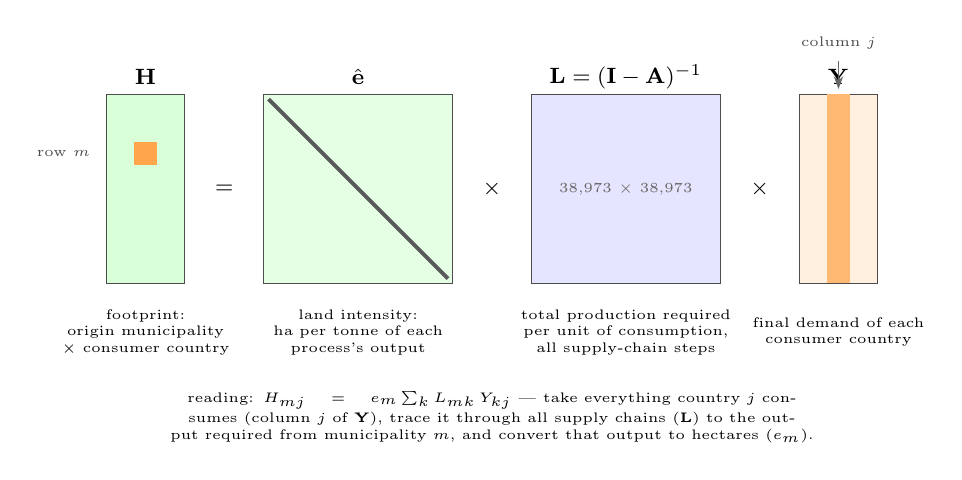
\begin{tikzpicture}[font=\footnotesize,
  lab/.style={font=\tiny, align=center}]
% ---- H ----
\draw[fill=green!15, draw=black!70] (0,0) rectangle (1.0,2.4);
\fill[orange!70] (0.35,1.5) rectangle (0.65,1.8); % H_mj
\node at (0.5,2.62) {$\mathbf{H}$};
\node[font=\tiny, anchor=east, black!70] at (-0.08,1.65) {row $m$};
\node[lab, text width=22mm] at (0.5,-0.62)
  {footprint:\\ origin municipality $\times$ consumer country};
% ---- = ----
\node at (1.5,1.2) {$=$};
% ---- e-hat ----
\draw[fill=green!10, draw=black!70] (2.0,0) rectangle (4.4,2.4);
\draw[black!65, line width=1.4pt] (2.06,2.34) -- (4.34,0.06);
\node at (3.2,2.62) {$\hat{\mathbf{e}}$};
\node[lab, text width=25mm] at (3.2,-0.62)
  {land intensity:\\ ha per tonne of each process's output};
% ---- times ----
\node at (4.9,1.2) {$\times$};
% ---- L ----
\draw[fill=blue!10, draw=black!70] (5.4,0) rectangle (7.8,2.4);
\node at (6.6,2.62) {$\mathbf{L}=(\mathbf{I}-\mathbf{A})^{-1}$};
\node[font=\tiny, black!60] at (6.6,1.2) {38{,}973 $\times$ 38{,}973};
\node[lab, text width=27mm] at (6.6,-0.62)
  {total production required per unit of consumption,\\ all supply-chain steps};
% ---- times ----
\node at (8.3,1.2) {$\times$};
% ---- Y ----
\draw[fill=orange!12, draw=black!70] (8.8,0) rectangle (9.8,2.4);
\fill[orange!55] (9.15,0) rectangle (9.45,2.4); % column j
\node at (9.3,2.62) {$\mathbf{Y}$};
\node[font=\tiny, black!70, above] at (9.3,2.85) {column $j$};
\draw[-{Stealth[length=1.6mm]}, black!60] (9.3,2.83) -- (9.3,2.47);
\node[lab, text width=22mm] at (9.3,-0.62)
  {final demand of each consumer country};
% ---- reading note ----
\node[align=center, font=\tiny, text width=110mm] at (4.9,-1.7)
  {reading: $H_{mj}=e_m\sum_k L_{mk}\,Y_{kj}$ --- take everything country $j$
   consumes (column $j$ of $\mathbf{Y}$), trace it through all supply chains
   ($\mathbf{L}$) to the output required from municipality $m$, and convert
   that output to hectares ($e_m$).};
\end{tikzpicture}
\caption{Linking consumption to land use. The footprint matrix $\mathbf{H}$
is the product of three objects: the land intensity of every process
($\hat{\mathbf{e}}$), the Leontief inverse summing all direct and indirect
production requirements ($\mathbf{L}$), and final demand by consumer country
($\mathbf{Y}$). The highlighted entry $H_{mj}$ is the soy area in
municipality $m$ embodied in country $j$'s consumption.}\label{fig:fpscheme}
\end{figure}

\subsubsection{Origin attribution and grid refinement}\label{subsubsec:attribution}
Each municipality is assigned to a biome by intersecting its interior point
with the IBGE 1:250{,}000 biome layer. The agricultural \emph{frontier} is
defined as the Amazon biome plus MATOPIBA (operationalized as the Cerrado
biome within Maranh\~ao, Tocantins, Piau\'i and Bahia), and a destination's
frontier share is the fraction of its origin footprint located in frontier
municipalities. For visualization, per-municipality embodied production can
optionally be distributed onto 30\,m MapBiomas soy pixels, each pixel of a
municipality carrying that municipality's per-pixel share for the given
consumer country; this refinement is illustrative and not load-bearing for
the results.

% ==================================================================
\subsection{Validation and benchmarking}\label{subsec:validation}
% ==================================================================
% Pipeline steps 10-11 (10_create_benchmarks.R, 11_analyse_benchmarks.R).

\subsubsection{Benchmark and baseline}\label{subsubsec:benchmarks}
The reconstructed origin-to-importer flows $X^p_{mj}$
(Section~\ref{subsubsec:exportlink}) are evaluated against the independent
Trase Brazil--soy dataset (v2.6.1), which links municipalities of production
to countries of first import using per-shipment customs and logistics records
\cite{godar2015sei,escobar2020trase}. As a second reference we construct a
\emph{pure-downscaling} baseline that uses no supply-chain structure at all:
national exports to each destination are allocated to municipalities in
proportion to their share in national soybean production --- the allocation
operator \eqref{eq:split} applied directly to bilateral exports. The
comparison thus brackets the model between an information-free lower bound and
a data-rich proprietary benchmark. All three sources are expressed in a common
unit by converting oil and cake flows to bean equivalents with the national
crush ratio (beans crushed per tonne of oil and cake produced). Trase flows
with unknown municipality of origin are excluded, destinations are harmonized
to the bilateral-trade classification, and the comparison sample comprises all
soy-producing municipalities crossed with the destinations recording positive
exports in both benchmark and model.

\subsubsection{Agreement metrics}\label{subsubsec:metrics}
Agreement is quantified on the municipality$\times$destination flow matrix by
the Pearson correlation coefficient $r$ (with Fisher 95\% confidence
intervals), the root-mean-square error and the root-mean-square logarithmic
error, computed (i) pooled over all pairs, (ii) per destination country, and
(iii) after aggregation to states. Because a municipality-level assignment can
be ``nearly right'' --- placing a flow in the neighbouring municipality of the
same production cluster --- all metrics are additionally computed on
neighbourhood-smoothed flows, using three spatial-weight schemes (first-order
contiguity, a 100\,km radius, and inverse distance, each raw and
row-standardized). Robustness of the conclusions across these tolerances
distinguishes genuine misallocation from boundary-precision noise.

\subsubsection{Volume--correlation decision rule}\label{subsubsec:volcorr}
Per-destination correlations are related to the destination's total import
volume to establish when subnational modelling adds information over pure
downscaling. Small trade volumes are handled by few shipments and carry no
recoverable spatial signal, so per-destination agreement degrades for all
methods below a volume floor (on the order of $10^3$\,t; Results). The
resulting decision rule --- model subnationally above the floor, downscale
below it --- is reported with the benchmark tables produced for every study
year.

% ==================================================================
\appendix
% ==================================================================
\section{Livestock system splits}\label{app:livestock}
Let $s^{k}_m$ denote municipality $m$'s share of system $k$ in the 2010
gridded-livestock rasters (area-weighted zonal sums, normalized across the
systems of each species); where a municipality reports a herd in the run year
but had no gridded animals in 2010, the state-mean share is substituted. Pigs
and chickens are split as
\begin{equation}
  N^{\mathrm{pig},k}_m=\text{pig}_m\,s^{\mathrm{Pg},k}_m,\quad
  N^{\mathrm{chk}}_{m,\mathrm{byd}}=\text{chicken}_m\,s^{\mathrm{Ch,Ext}}_m,\quad
  N^{\mathrm{chk}}_{m,\mathrm{lay}}=\text{chicken\_layer}_m\,s^{\mathrm{Ch,Int}}_m,
\end{equation}
with broilers
$N^{\mathrm{chk}}_{m,\mathrm{bro}}=(\text{chicken}_m-\text{chicken\_layer}_m)\,s^{\mathrm{Ch,Int}}_m$
(or $\text{chicken}_m\,s^{\mathrm{Ch,Int}}_m$ where layers are unreported).
Feedlot cattle are the 2006 census counts scaled by the national confinement
growth factor for the run year (e.g.\ $4.38/3.46\approx1.27$ for 2013, from
ABIEC/Athenagro), holding the municipal pattern fixed. The remaining cattle
are split into grassland/mixed systems by the raster shares
$s^{\mathrm{Catt},u}_m$, $u\in\{\mathrm{gra,mix}\}$, with dairy identified by
milked cows and meat as the residual:
\begin{align}
  N^{\mathrm{cattle}}_{m,u,\mathrm{dair}}&=\text{cattle\_milked}_m\,s^{\mathrm{Catt},u}_m,\\
  N^{\mathrm{cattle}}_{m,u,\mathrm{meat}}&=\big(\text{cattle}_m-\text{cattle\_milked}_m-N^{\mathrm{cattle,flot}}_m\big)\,s^{\mathrm{Catt},u}_m .
\end{align}
Buffalo use the municipal milked-cow ratio
$\rho_m=\text{cattle\_milked}_m/\text{cattle}_m$ as the dairy proxy,
\begin{equation}
  N^{\mathrm{buf}}_{m,u,\mathrm{dair}}=\text{buffalo}_m\,\rho_m\,s^{\mathrm{Buff},u}_m,
  \qquad
  N^{\mathrm{buf}}_{m,u,\mathrm{meat}}=\text{buffalo}_m\,(1-\rho_m)\,s^{\mathrm{Buff},u}_m .
\end{equation}
Each species' subsystems partition its reported herd exactly, e.g.\
$\text{cattle}_m=N^{\mathrm{cattle,flot}}_m+\sum_{u}\sum_{v\in\{\mathrm{dair,meat}\}}N^{\mathrm{cattle}}_{m,u,v}$.

%%%%%%%%%%%%%%%%%%%%%%%%%%%%%%%%%%%%%%%%%%%%%%%%%%%%%%%%%%%%%%%%%%%%%%
\bibliography{refs}%
%%%%%%%%%%%%%%%%%%%%%%%%%%%%%%%%%%%%%%%%%%%%%%%%%%%%%%%%%%%%%%%%%%%%%%

\end{document}
